\documentclass[times, utf8, seminar]{fer}
\usepackage{booktabs}
\usepackage{algorithm}
\usepackage{algpseudocode}
\usepackage{amsmath}
\usepackage{float}
\usepackage[activate={true,nocompatibility},final,tracking=true,kerning=true,spacing=true,factor=1100,stretch=10,shrink=10]{microtype}
\microtypecontext{spacing=nonfrench}
\begin{document}

% TODO: Navedite naslov rada.
\title{Računanje najduljeg zajedničkog prefiksa temeljeno na BWT}

% TODO: Navedite vaše ime i prezime.
\author{Lovre Mrčela, Ana Škaro, Ante Žužul}

% TODO: Navedite ime i prezime mentora.
\voditelj{doc.dr.sc. Mirjana Domazet-Lošo}

\maketitle

\tableofcontents

\chapter{Uvod}

Bioinformatika se bavi analizom sekvenci genoma. U toj analizi, mnogi algoritmi koriste sufiksna polja i polja najduljeg zajedničkog prefiksa. Cilj ovog projekta bio je implementirati algoritme 1 i 2 iz rada \cite{beller2013}, uz korištenje gotove knjižnice za izgradnju sufiksnog polja. Implementaciju je potom bilo potrebno testirati s gotovom knjižnicom koja sadržava implementaciju stabla valića, a napravljena je i naša implementacija stabla valića, odnosno njegova funkcija rang (engl. \textit{rank}). Konačno rješenje je trebalo biti uspoređeno s rezultatima iz studentskog rada \cite{studenti2016}. Kao ulazni niz koristio se genom Escherichie coli.

\chapter{Algoritmi}
U svom radu \cite{beller2013} navode kako porast informacija koje se u novije doba mogu dobiti analizom sekvenci DNK, zahtijevaju podatkovne strukture koje zauzimaju manje prostora. Jedna od njih je stablo valića niza transformiranog Burrows--Wheelerovom transformacijom (BWT). Opisani postupak odvija se u sljedećim koracima: 1) niz se transformira Burrows--Wheelerovom transformacijom, 2) transformirani niz se pohranjuje u stablo valića, 3) stablo valića omogućuje pretraživanje unatrag na originalnom nizu.
Mnogi algoritmi za sekvenciranje koriste najdulji zajednički prefiks (engl. \textit{longest common prefix, LCP}), \cite{beller2013} u svom radu navode kako većina postojećih postupaka za izračun LCP-polja (engl. \textit{LCP-array}) prvo gradi sufiksno polje, a potom u linearnom vremenu dolazi do LCP-polja. Zbog toga, oni predlažu algoritam koji radi direktno nad BW transformiranim nizom znakova, a ne nad sufiksnim poljem. Taj algoritam ima vremensku složenost $O$(n$\log\sigma$), gdje je $\sigma$ veličina abecede. U nastavku je opisan ovaj postupak, temeljen na algoritmima 1 i 2 iz navedenog rada te podatkovne strukture potrebne za njegovu implementaciju.

\section{Podatkovne strukture}

\subsection{Stablo valića}
\label{stablo_valica_def}
Stablo valića (engl. \textit{wavelet tree}) omogućuje pretraživanje unatrag u vremenskoj složenosti od $O$(log$\sigma)$ po koraku. Za razumijevanje strukture potrebno je prvo objasniti nekoliko pojmova. Poredana abeceda $\Sigma$ je polje veličine $\sigma$, tako da su znakovi poredani uzlazno u polje $\Sigma$[1...$\sigma$], primjerice $\Sigma$[1]=$\$$ < $\Sigma$[2] < ... < $\Sigma[\sigma]$. Interval [l...r] je \textit{abecedni interval}, ako je to podinterval intervala [1...$\sigma$]. Za abecedni interval [l...r], niz znakova $BWT^{[l..r]}$ se dobije iz BW transformiranog niza znakova BWT od S, brisanjem svih znakova u BWT koji ne pripadaju pod-abecedi $\Sigma$[l...r] od $\sigma$[1...$\sigma$].
Stablo valića niza znakova BWT izgrađeno nad abecedom $\Sigma$[1...$\sigma$] je balansirano binarno stablo pretraživanja (engl. \textit{balanced binary search tree}) definirano u nastavku. Svaki čvor $v$ odgovara nizu znakova BWT$^{[l..r]}$, gdje je [l..r] abecedni interval. Korijen stabla odgovara nizu znakova BWT = BWT$^{[1..\sigma]}$. Ako je l=r, onda taj čvor $v$ nema djece. Inače, svaki čvor $v$ ima dvoje djece: \textbf{lijevo dijete} odgovara nizu znakova BWT$^{[l..m]}$, dok \textbf{desno dijete} odgovara nizu znakova BWT$^{[m+1..r]}$, gdje je m = $\lfloor\frac{l+r}{2}\rfloor$. U ovom slučaju $v$ sadrži bit vektor (engl. \textit{bit vector}) B$^{[l..r]}$, čiji je i-ti element 0 ako je i-ti znak u BWT$^{[l..r]}$ iz pod-abecede $\Sigma$[l..m], a 1 ako je iz pod-abecede $\Sigma$[m+1..r]. Drukčije rečeno, element bit vektora je 0 ako odgovarajući znak pripada lijevom podstablu, a 1 ako odgovarajući znak pripada desnom podstablu. Izgradnja stabla valića objašnjena je na primjeru u poglavlju \ref{chptr_primjer}.

Svaki vektor B u stablu predprocesira se tako da se upiti \textit{rank$_{0}$(B,i)} i \textit{rank$_{1}$(B,i)} mogu odgovoriti u konstantnom vremenu, gdje \textit{rank$_{b}$(B,i)} predstavlja broj pojavljivanja bita \textit{b} u B[1..i]. Stablo valića ima visinu $O(\log\sigma$). S obzirom da je u implementaciji dovoljno spremiti samo bit vektore, stablo valića zahtijeva samo n$\log\sigma$ bitova prostora i $O(nlog\sigma$) bitova za podatkovne strukture koje podržavaju rang upite u konstantnom vremenu.

\subsection{Sufiksno polje}
Sufiksno polje (engl. \textit{suffix array, SA}) niza znakova S je cjelobrojno polje u intervalu od 1 do \textit{n} koje određuje leksikografski poredak \textit{n} sufiksa niza znakova S. Točnije, sufiksno polje SA zadovoljava: S$_{SA[1]}$ < S$_{SA[2]}$ < ... < S$_{SA[n]}$, gdje S$_i$ označava i-ti sufiks S[i..n] niza znakova S. 

\subsection{Burrows--Wheelerova transformacija (BWT)}

\label{BWT_def}
Burrows--Wheelerova transformacija ili BWT, pretvara niz znakova S u niz znakova BWT[1..n], definiran kao: 
\[
BWT[i]=\begin{cases}
	S[SA[i]-1], & \text{ako } SA[i]\neq 1 &
	\$, & \text{inače}.
\end{cases}
\]

\section{Izračunavanje LCP na temelju BWT}
\label{[algoritmi_def]}
Autori u radu \cite{beller2013} koriste dva algoritma kako bi izgradili LCP polje i naš osnovni zadatak unutar ovog projekta bio je upravo implementacija tih dvaju algoritama.
Prema prvom algoritmu koji su autori predložili, za jedan $\omega$-interval[i..j], funkcija \textit{getIntervals([i..j])} vraća listu svih \textit{c$\omega$}-intervala. To ustvari znači da se unutar intervala [i..j] pronađu svi znakovi abecede $\Sigma$, koji se potom poredaju leksikografski te se za svaki od znakova računa njegov $\omega$-interval. Na poslijetku, funkcija vraća onoliko c$\omega$ intervala koliko ima jedinstvenih znakova u intervalu [i..j].
Postupak započinje $\omega$ intervalom [i..j] u korijenu stabla valića te se nastavlja spuštati u dubinu (kao DFS (engl. \textit{depth-first search}) algoritam).
Dok se nalazi u trenutnom čvoru, algoritam postavlja rang upit stablu valića (složenost upita je konstantna!), kako bi došao do broja b$_{0}$ - a$_{0}$. Taj broj predstavlja nule u bit vektoru trenutnog čvora \textit{v} unutar trenutnog intervala. Ako je ta vrijednost pozitivna u BWT[i..j] se nalaze znakovi koji pripadaju lijevom podstablu čvora \textit{v} i algoritam nastavlja rekurzivno pozivanje unutar lijevog djeteta čvora \textit{v}. Isto tako, ako je broj jedinica pozitivan (b$_1$ - a$_1$), onda se algoritam nastavlja odvijati u desnoj grani. Algoritam se zaustavlja kad se za trenutni interval [p..q] dosegne list stabla koji odgovara znaku \textit{c}. Tada je c$\omega$-interval [C[c]+p..C[c]+q], gdje je C[c] zbroj rangova svih elemenata iz poredane abecede koji su leksikografski manji od znaka c. Vremenska složenost ovog postupka je $O$(\textit{k}log$\sigma$), gdje je k duljina liste c$\omega$-intervala.

Kao što je već rečeno, \textbf{algoritam 2} se oslanja na algoritam 1. Svi elementi polja LCP[1..n+1] se inicijalno postavljaju na neku nemoguću vrijednost, npr. $\perp$, osim prvog i zadnjeg elementa koji poprimaju vrijednost -1. Jedan red (engl. \textit{queue}) sadržava parove (interval,\textit{l}). Na početku rada algoritma u redu se nalazi samo interval [1..n], a \textit{l} vrijednost je postavljena na 0. Algoritam potom skida iz reda interval (po principu FIFO, dok god se red ne isprazni), te pozivom metode \textit{getIntervals} prvog algoritma dobiva listu c$\omega$-intervala za dani interval. Za svaki interval [lb..rb] iz liste c$\omega$-intervala gleda se je li vrijednost polja LCP[rb+1] nepostavljena (iznosi $\perp$) te ako jest, taj interval [lb..rb] se dodaje u red, a njegova \textit{l} vrijednost se povećava za 1 u odnosu na \textit{l} vrijednost intervala koji je posljednji skinut iz reda. Također, vrijednost LCP[rb+1] se postavlja na tu posljednju \textit{l} vrijednost. 

\begin{algorithm}[H]
\caption{prema \cite{beller2013}}
\label{alg1}
\begin{algorithmic}
\Function{getIntervals}{[i..j]}
\State $list \gets$ []
\State getIntervals'([i..j],[1..$\sigma$],list)
\State \Return $list$
\EndFunction

\Function{getIntervals'}{[i..j],[l..r],list}
\If {$l = r$}
	\State $c \gets \Sigma[l]$
	\State $add(list, [C[c]+i..C[c]+j)$ 
\Else
	\State $(a_0,b_0) \gets (rank_0(B^{[l..r]},i-1),rank_0(B^{[l..r]},j))$
	\State $(a_1,b_1) \gets (i-1-a_0,j-b_0)$
	\State $m \gets \lfloor\frac{l+r}{2}\rfloor$ 
	\If {$b_0 > a_0$}
	\State \textit{getIntervals'}([a$_0$+1..b$_0$],[l..m],list)
	\EndIf
	\If{$b_1 > a_1$}
	\State \textit{getIntervals'}([a$_1$+1...b$_1$],[m+1..r],list)
	\EndIf
\EndIf

\EndFunction
\end{algorithmic}
\end{algorithm}



\begin{algorithm}[H]
\caption{prema \cite{beller2013}}
\label{alg2}
\begin{algorithmic}
\State inicijalizacija polja LCP[1..n+1]  /* npr. LCP[i]=$\perp$ za sve $1 \leq i \leq n+1$ */
\State LCP[1] $\gets$ -1; LCP[n+1] $\gets$ -1
\State inicijaliziraj prazni red
\State dodaj (<[1..n],0>) u red q
\While{q nije prazan}
\State <[i..j],$l$> $\gets q.pop()$
\State list $\gets$ \textit{getIntervals}([i..j])
\For{\textbf{each}\texttt{[lb..rb] \textbf{in} \textit{list}}}
\If{LCP[rb+1]=$\perp$}
\State $q.push(<[lb..rb],l+1>)$
\State LCP[rb+1] $\gets l$
\EndIf
\EndFor

\EndWhile
\end{algorithmic}
\end{algorithm}

\subsection{Primjer}
\label{chptr_primjer}
U nastavku je dan primjer rada algoritma na stringu S$_u$=\textit{annasanannas}. preuzet iz prošlogodišnjeg rada studenata \cite{studenti2016}.

Prvo se iz niza gradi sufiksno polje. 


\begin{enumerate}
  \item Na kraj niza znakova S$_u$ dodaje se znak \$ (najmanji znak abecede) Sada imamo niz S = annasanannas\$.
  \item Svakom sufiksu niza S pridružuju se indeksi od 1 do \textit{n}, počevši od najduljeg. Ovo je prikazano u \textbf{tablici \ref{tablePrimjer1}}
  \item Sufiksi se potom poredaju leksikografski, čime nastaje sufiksno polje SA = [13, 6, 8, 1, 11, 4, 7, 10, 3, 9, 2, 12, 5]. Ovo je prikazano u \textbf{tablici \ref{tablePrimjer2}}.
  \item Iz polja SA se prema formuli navedenoj u \ref{BWT_def} izračunava Burrows-Wheelerov niz BWT[1..n]. 
  Rezultat je prikazan u 4. stupcu \textbf{tablice \ref{tablePrimjer2}}. 
  Npr. BWT[10]=S[SA[10]-1]=S[9-1]=S[8]=a.
  \item Iz Burrows-Wheelerove transformacije niza znakova, gradi se stablo valića. Poredana abeceda u ovom primjeru ima 4 znaka $\Sigma$[1..4]=\$ans. U korijen stabla se stavlja bit vektor dobiven kodiranjem niza BWT prema pravilu opisanom u poglavlju \ref{stablo_valica_def}. Abeceda se podijeli na dva dijela, u ovom slučaju: $\Sigma$[1..2]=\$a i $\Sigma$[3..4]=ns. Znakovi u prvoj polovini se kodiraju vrijednošću 0, a ostali 1. Ovaj postupak se ponavlja sve dok se u čvoru ne nalaze samo jednaki znakovi. Nastalo stablo može se vidjeti na slici \ref{fig:stablo}.
  \item U ovom koraku može započeti konstrukcija polja najdužih zajedničkih prefiksa, za što se koriste algoritmi 1 i 2 iz rada \cite{beller2013} opisani u poglavlju \ref{[algoritmi_def]}.
  \begin{enumerate}
  \item Inicijalizacija polja LCP i reda Q:
  \begin{itemize}
  \item LCP = [-1,$\perp,\perp,\perp,\perp,\perp,\perp,\perp,\perp,\perp,\perp,\perp,\perp, \perp$, -1]
  \item red Q = [<[1..13],0>]
   \end{itemize}
   \item Uklanjanje elementa iz reda Q po FIFO principu te izračunavanje c$\omega$-intervala za taj interval pomoću funkcije \textit{getIntervals}.
   \begin{itemize}
   \item Indeks početka intervala dobiva se po formuli \textit{rang}(c,i-1)+C[c]+1. Indeks kraja intervala dobiva se po formuli C[c]+\textit{rang}(c,j).Funkcija \textit{rang(a,k)} vraća broj pojavljivanja znaka \textit{a} do \textit{k}-tog indeksa u polju. 
   \item Interval $I$ = [i..j]=[1..13]. 
   \item Znakovi abecede iz intervala $I$ se poredaju leksikografski. Ima onoliko c$\omega$-intervala koliko je i jedinstvenih znakova.
   \item $C$ = [0,1,6,11]
   \item U $I$ se nalaze \textbf{svi} znakovi abecede (\$,a,n,s). Algoritam prolazi svaki od znakova i računa njegov interval prema formuli navedenoj iznad.
   \item  [\textit{rang}('\$',0)+C['\$']+1..C['\$']+\textit{rang}('\$',13)]=[0+0+1..+0+1]=[1..1]
   \item [\textit{rang}('a',0)+C['a']+1..C['a']+\textit{rang}('a',13)]=[0+1+1..+1+5]=[2..6]
   \item
   [\textit{rang}('n',0)+C['n']+1..C['n']+\textit{rang}('n',13)]=[0+6+1..+6+5]=[7..11]
   \item
   [\textit{rang}('s',0)+C['s']+1..C['s']+\textit{rang}('s',13)]=[0+11+1..+11+2]=[12..13]
   \item Konačno, povratna vrijednost \textit{getIntervals} je lista c$\omega$-intervala: \newline [[1..1],[2..6],[7..11],[12..13]]. Za svaki od tih intervala se potom provjerava vrijednost LCP[rb+1] te se postupa sukladno koracima u pseudokodu algoritma 2.
   \end{itemize}
     \item Konačna vrijednost polja LCP, nakon što algoritam završi s radom je: 
       	LCP = [-1,0,2,5,1,2,0,2,3,1,4,0,1,-1].
  \end{enumerate}

\end{enumerate}

\begin{figure}
	\begin{center}
		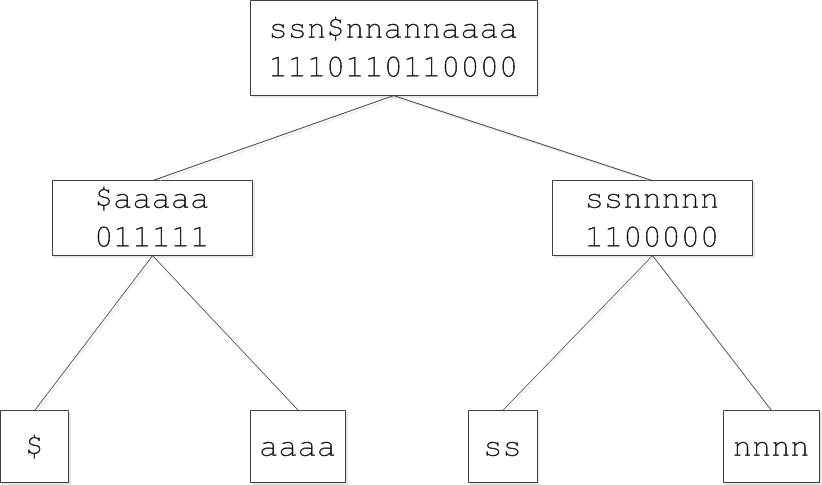
\includegraphics[width=\columnwidth]{wavelet_tree.png}
		\caption{Slika prikazuje izgled stabla valića za dani primjer.}
		\label{fig:stablo}
	\end{center}
\end{figure}

\begin{table}
\caption{Pridruživanje indeksa sufiksima niza S, počevši od najduljeg.}
\label{tablePrimjer1}
\begin{center}
\begin{tabular}{ll}
\toprule
i & S$_{SA}$[i] \\
\midrule
1 & annasanannas\$ \\
2 & nnasanannas\$ \\
3 & nasanannas\$ \\
4 & asanannas\$ \\
5 & sanannas\$ \\
6 & anannas\$ \\
7 & nannas\$ \\
8 & annas\$ \\
9 & nnas\$ \\
10 & nas\$ \\
11 & as\$ \\
12 & s\$ \\
13 & \$ \\
\bottomrule
\end{tabular}
\end{center}
\end{table}


\begin{table}
\caption{Sufiksi su poredani leksikografski, a njihovi indeksi čine sufiksno polje SA.}
\label{tablePrimjer2}
\begin{center}
\begin{tabular}{rrll}
\toprule
i & SA[i] & S$_{SA}$[i] & BWT[i] \\
\midrule
1 & 13 & \$ & s\\
2 & 6 &  anannas\$ & s \\
3 & 8 & annas\$ & n \\
4 & 1 & annasanannas\$ & \$ \\
5 & 11 & as\$ & n \\
6 & 4 & asanannas\$ & n \\
7 & 7 & nannas\$ & a\\
8 & 10 & nas\$ & n\\
9 & 3 & nasanannas\$ & n \\
10 & 9 & nnas\$ & a\\
11 & 2 & nnasanannas\$ & a \\
12 & 12 & s\$ & a\\
13 & 5 & sanannas\$ & a \\
\bottomrule
\end{tabular}

\end{center}

\end{table}



\chapter{Rezultati}

Nakon implementacije opisanih algoritama zadatak je bio usporediti ih s rezultatima studentskog rada \cite{studenti2016} \footnote{Cijeli rad i implementacija su dostupni na \textit{https://github.com/wissil/LCP\_BWT}.} te s originalnom implementacijom Simona Goga (prema radu \cite{beller2013}) na ulaznom nizu koji pripada genomu Escherichie coli. Usporedba je napravljena koristeći alat \textit{cgmemtime}\footnote{Alat \textit{cgmemtime} se može pronaći na \textit{https://github.com/isovic/cgmemtime}.} na računalu sa sustavom Arch Linux. Napominjemo da smo implementaciju Simona Goga kojoj smo testirali vrijeme izvođenja preuzeli smo iz rada studenata.

Kako možemo vidjeti u tablici \ref{tableRezultatiVrijeme} i na slici \ref{fig:graf1}, naša implementacija se ponašala bolje u odnosu na implementaciju studenata \cite{studenti2016} i to za čak 8 do 9 puta bolje na duljim nizovima znakova. U odnosu na originalnu implementaciju algoritma, naš je algoritam bio sporiji (što je i u redu za očekivati), ali tek oko 1.5 puta. Dobro je primijetiti da se razlike među algoritmima osjetno primjećuju tek na nizovima iznad deset tisuća (10000) znakova. 

Što se tiče potrošnje memorije, prikazane u tablici \ref{tableRezultatiMemorija} i na slici \ref{fig:graf2}, naš algoritam se na nizovima do 250000 znakova ponašao bolje od rada studenata, a kasnije im je bio relativno blizu. Originalna implementacija Simona Goga na kraćim nizovima treba više memorijskog prostora, ali zato pri povećanju ulaznog niza s milijun (1000000) znakova na puni genom Escherichie Coli (4639211) znakova ima porast od tek 2-3 puta, dok naš algoritam zahtjeva gotovo 5 puta više memorije pri takvom skoku.

\section{Tablice i grafovi}
 U nastavku su prikazane tablice i grafovi usporedbe vremena izvođenja i zauzeća memorije različitih implementacija algoritma.
\begin{table}
\caption{Rezultati usporedbe vremena izvođenja naše implementacije algoritma i implementacije iz rada \cite{studenti2016} te originalne implementacije Simona Goga.}
\label{tableRezultatiVrijeme}
\begin{center}
\begin{tabular}{rlll}
\toprule
Duljina ulaznog & Naša & Implementacija & Originalna implementacija \\
niza   [znak] & implementacija [s] & \cite{studenti2016} [s] &  Simona Goga [s]\\
\midrule
1000 & 0.000 & 0.023 & 0.016\\
5000 & 0.000 &  0.039 & 0.031 \\
10000 & 0.008 & 0.070 & 0.023 \\
100000 & 0.062 & 0.703 & 0.055 \\
250000 & 0.18 & 1.703 & 0.117 \\
500000 & 0.391 & 3.398 & 0.258\\
750000 & 0.648 & 5.078 & 0.398\\
1000000 & 0.805 & 6.625 & 0.469 \\
4639211 & 4.000 & 34.438 & 3.031\\
\bottomrule
\end{tabular}
\end{center}
\end{table}

\begin{figure}
 \begin{center}
 		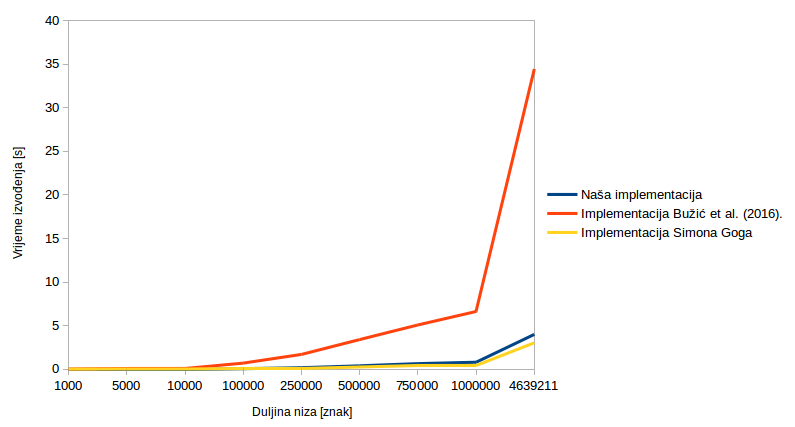
\includegraphics[width=\columnwidth]{prvi.png}
 		\caption{Graf prikazuje rezultate usporedbe vremena izvođenja algoritma prema tablici \ref{tableRezultatiVrijeme}}
 		\label{fig:graf1}
 \end{center}
\end{figure}


\begin{table}
\caption{Rezultati usporedbe zauzeća memorije naše implementacije algoritma i implementacije iz rada \cite{studenti2016} te originalne implementacije Simona Goga.}
\label{tableRezultatiMemorija}
\begin{center}
\begin{tabular}{rlll}
\toprule
Duljina ulaznog & Naša & Implementacija & Originalna implementacija \\
niza   [znak] & implementacija [KiB] & \cite{studenti2016} [KiB] &  Simona Goga [KiB]\\
\midrule
1000 & 3476 & 6336 & 9532\\
5000 & 3732 &  6392 & 12308 \\
10000 & 3592 & 6400 & 12320 \\
100000 & 6768 & 7736 & 12360 \\
250000 & 11992 & 11996 & 12848 \\
500000 & 20880 & 20644 & 13816\\
750000 & 30736 & 30424 & 14564\\
1000000 & 38532 & 38172 & 15216 \\
4639211 & 178172 & 170020 & 43516\\
\bottomrule
\end{tabular}
\end{center}
\end{table}

\begin{figure}
 \begin{center}
 		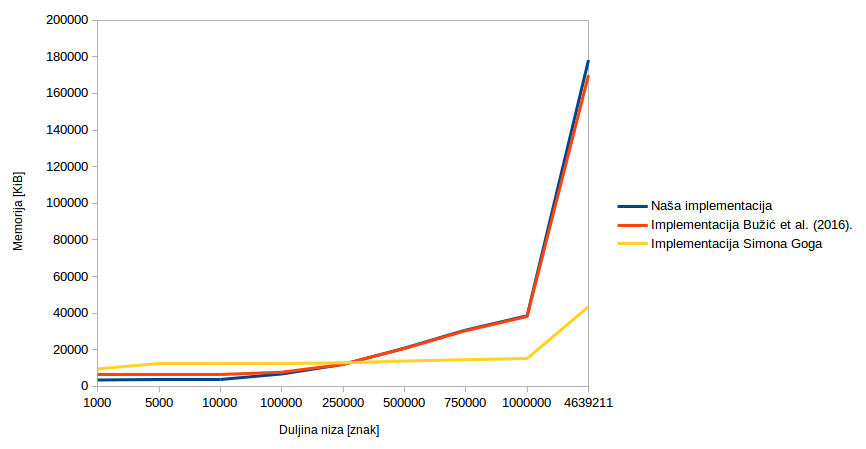
\includegraphics[width=\columnwidth]{drugi.png}
 		\caption{Graf prikazuje rezultate usporedbe zauzeća memorije prilikom izvođenja algoritma prema tablici \ref{tableRezultatiMemorija}}
 		\label{fig:graf2}
 \end{center}
\end{figure}


\chapter{Zaključak}

Organske molekule, npr. DNK, proteini, koji su predmeti proučavanja bioinformatike, predstavljeni su nizovima znakova. Ti nizovi znakova su velikih duljina pa njihovo pretraživanje i analiza zahtijeva korištenje optimiziranih algoritama i struktura podataka. Jedna od stvari koja pomaže tim postupcima je polje najdužih sajedničkih prefiksa (LCP-polje). LCP polje može se izgraditi u složenosti $O$(n$\log\sigma$), gdje je $\sigma$ veličina abecede, kako je pokazano radom \cite{beller2013}. U našem radu je uspješno implementiran predloženi algoritam koji uključuje izgradnju stabla valića nad Burrows--Wheelerovim transformiranim nizom znakova. Naš algoritam se bolje nosi s dugim nizovima od prethodno implemetiranih studentskih algoritama. Ipak, još uvijek je nešto lošiji od implementacije Simona Goga kad se radi o duljim nizovima znakova. Kao najveći nedostatak možemo primijetiti nagli porast zauzeća memorije pri povećanju ulaznog niza s milijun na preko 4.5 milijuna znakova. Originalna implementacija na manjim nizovima troši više memorije od naše, no zato je porast potrošnje znatno stabilniji.

\bibliography{literatura}
\bibliographystyle{fer}

\chapter{Sažetak}
Ovaj rad je napravljen kao projekt iz predmeta Bioinformatika diplomskog studija računarstva na Fakultetu elektrotehnike i računarstva, sveučilišta u Zagrebu. Cilj projekta bila je implementacija algoritama za izračun polja najdužih zajedničkih prefiksa (LCP-polja) iz rada \cite{beller2013}, uz korištenje gotove knjižnice za izgradnju sufiksnog polja. Implementacija je testirana i uz gotovu i uz vlastitu implementaciju stabla valića. Konačno rješenje je uspoređeno s rezultatima iz studentskog rada \cite{studenti2016} naspram kojih je dalo bolje rezultate po pitanju vremena izvođenja i zauzeća memorije.

\end{document}
